\begin{document}
	
	The IC buck converter replaces the entire circuit designed above and replaces it with an IC package. The filter, however still needed to be built around the load. The load used a potentiometer tied to the feedback pin of the IC to enable a variable voltage on the load. Certain limitations of the IC needed to be considered when designing the circuit. A block diagram of a typical Buck converter using this IC is provided below. 
	
	\begin{figure}[H]
		\centering
		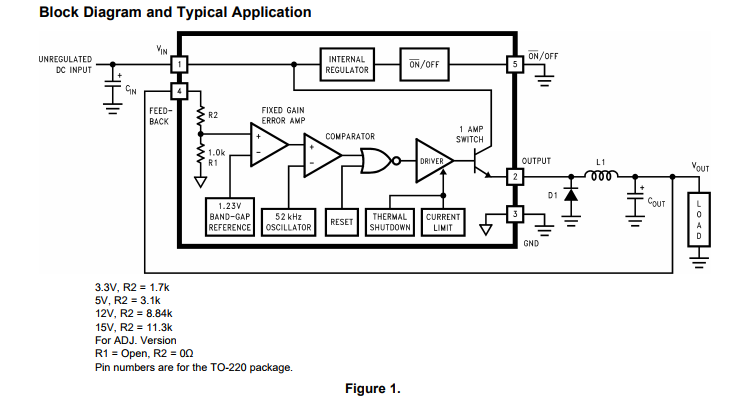
\includegraphics[width=.6\textwidth]{CircuitDevelopment/ICblock.png}
		\caption{IC Buck converter block diagram [5]}
		\label{fig:icblock}
	\end{figure}
	
	The block diagram above shows the inside of the IC used in designing the final Buck Converter.
	
	
	
	
	
\end{document}